\subsection{Entity-Relationship Schema}

%The ER schema needs to be completed with attributes, color for different parts of the application and name for two relations
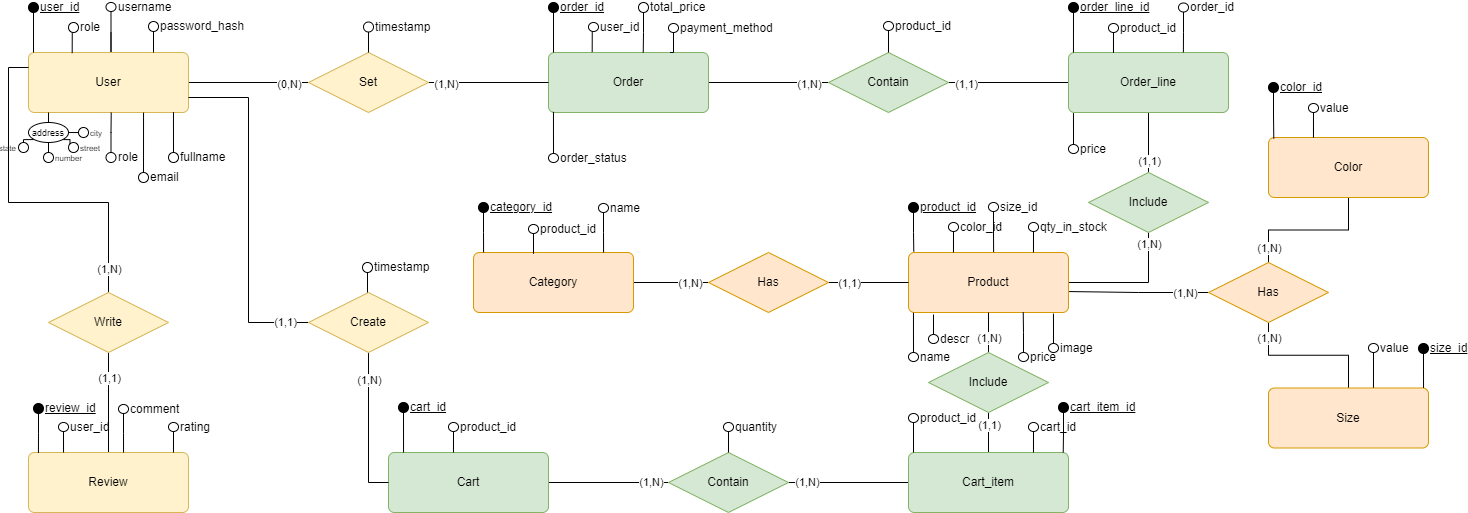
\includegraphics[width=\columnwidth]{images/wave_er.png}

\noindent The entity-relationship contains 9 entities:

%The design of the database was rethinked so this description is not perfectly matching the actual ER Diagram and has to be refactored
% \begin{itemize}
%     \item  \textbf{User}: the entity represent the user that can access the application. The primary
%     key (\textbf{user_id}) is an integer with auto-increment. Then it has the subsequent attributes:
%      \begin{itemize}
%         \item  \textbf{username}: used to identify the user inside the application;
%         \item  \textbf{password_hash}: used to memorize the hash of the password. It is saved only the hash for security reasons;
%         \item  \textbf{email}: used to register the user in the application. With the password is necessary to sign-up and sign-in;
%         \item  \textbf{full_name}: personal information of the user;
%         \item  \textbf{address}: necessary for order information
%         \item  \textbf{role}: this attribute is an Enum and identifies a specific user. There are 2 different type of users
%         \begin{itemize}
%             \item \textbf{admin} 
%             \item \textbf{base}
%         \end{itemize}
%      \end{itemize}
    
%    \item  \textbf{Shopping_Cart}: the entity represents the cart in which the products, waiting to be purchased by a \textbf{user}, are inserted. The Primary Key is \textbf{cart_id}.
%    \item \textbf{Order}: the entity represent a order done by a user. It has the subsequent attrbutes:
%     \begin{itemize}
%         \item \textbf{order_date}: it stores the date of the order in which the user complete the purchased
%         \item \textbf{total_price}: the amount of the purchase done by the user
%         \item \textbf{payment_status}: the status of the purchase it can be one of the following
%         \begin{itemize}
%             \item Pending
%             \item Complete
%             \item Failed
%             \item Cancelled
%         \end{itemize}
%     \end{itemize}
%     \item \textbf{Line_Item}: this entity represent a product inside the cart and inside an order. The Primary Key is \textbf{line_item_id}, it has the subsequent attributes:
%     \begin{itemize}
%         \item quantity
%         \item price
%     \end{itemize}
%     \item \textbf{Product_Review}: this entity represent a review written by a user for a specific product 
%     \item \textbf{Product}: this entity represent a product available for purchase by an user.The Primary Key is \textbf{product_id}, it has the subsequent attributes:
%     \begin{itemize}
%         \item name
%         \item description
%         \item price
%         \item stock_qty
%         \item type
%         \item size
%         \item color 
%         \item brand 
%     \end{itemize}
%     \item \textbf{Category}: describes the category of a specific product, the primary
%     key is an integer with auto-increment. There are two additional attributes: the category_description and the category_name.
% \end{itemize}